\chapter{Video data format}
\renewcommand{\baselinestretch}{\mystretch}
\label{chap:Video}
%\setlength{\parindent}{0pt}

With the implementation of \texttt{VixenConsole}, the process of designing and pre-rendering (exporting) the sequence on Vixen application then playback later using \texttt{VixenConsole} became very similar to the process of video editing and playback. Therefore, it may be beneficial to add support for video sequence format.

\section{Implementation}

The open source \texttt{ffmpeg} framework \cite{ffmpeg} was used for video processing. The open source nature ensures up-to-date version of \texttt{ffmpeg} is available on all testing platforms.

The \texttt{ffmpeg} framework uses the C programming language for its API. The complicity of different data structures used by \texttt{ffmpeg} results in no up-to-date C\# wrapper API available for use directly. Therefore, an intermediate wrapper layer between Vixen and \texttt{ffmpeg} was developed to encapsulate all complex \texttt{ffmpeg} routines using C.

The development of video integration was separated into multiple steps. Firstly, several C programs were developed to test individual video processing functions including video encoding, video decoding, stream muxing and metadata retrieve. Afterwards, working code segments were combined into a dynamic library, with a simplified API suitable for C\#. A C\# wrapper class was then developed using the \texttt{InterOp} service \cite{interop}, together with another C\# program for testing video encoding and decoding. After all these small testing programs had been confirmed working, the C\# wrapper was finally integrated into Vixen with the playback engine. The playback engine checks for input file extension to determine whether to load the file as exported ``Raw'' sequence or video file.

To ensure lossless transcoding from the ``Raw'' sequence to video stream, the transcoding programs were tested by encoding example sequences to video then decoded back to another sequence. The two sequences were then compared for any difference, using the GNU \texttt{diff} tool \cite{diff}. Makefile was used for automated compiling and testing.

To minimise number of files needed for playback, the optional audio file was muxed together with the video stream, and the network configuration XML file was stored directly as string literal in video metadata field ``comment'', as shown by \fref{fig:video-info}.

\begin{figure}[t]
  \centering
  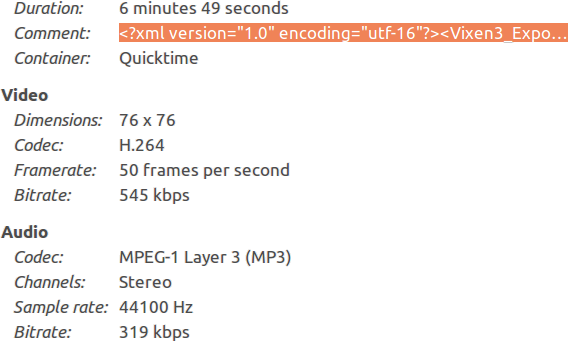
\includegraphics[width=0.7\textwidth]{Figs/video_info.png}
  \caption{\footnotesize Media information of an example video sequence}
  \label{fig:video-info}
\end{figure}

In the playback engine, video frames will be transformed to controller data frames for rendering. However, the existing audio rendering engine \texttt{FMOD} from Vixen only supports media file playback. The required functionality of playing decoded data frames was not available from its C\# API. To resolve this issue, C code for operating a newer version of \texttt{FMOD} was added to the wrapper library. The playback engine transfers the decoded audio frame back to the wrapper library for audio playback.

\section{Benefits and limitations}

The first noticeable benefit was reduction in sequence file size. The ``Raw'' sequence format was implemented without any compression algorithm, always has a size linear to total sequence time and channel count. The video formats reduced the sequence size to around $\frac{1}{10}$ of the ``Raw'' sequence. \tref{tbl:size} compares file sizes in different formats of the same example sequence.

\begin{table}[t]
  \centering
  \begin{tabular}{l|l|l}
    \hline
    \textbf{Type} & \textbf{Sequence size} & \textbf{With audio} \\
    \hline
    Editable sequence                     & 8.88 MiB  & 24.4 MiB  \\ \hline
    50 fps exported \texttt{Raw} sequence & 337 MiB   & 352 MiB   \\ \hline
    50 fps \texttt{rgb24} encoded video   & 26.6 MiB  & 42.5 MiB  \\ \hline
    50 fps \texttt{yuv444p} encoded video & 26.6 MiB  & 42.5 MiB  \\ \hline
    50 fps \texttt{yuv420p} encoded video & 18.2 MiB  & 34.1 MiB  \\ \hline
  \end{tabular}
  \caption{\footnotesize File size comparison of different formats}
  \label{tbl:size}
\end{table}

Using the video format, the exported sequence, audio and configuration information are combined into a single file. This reduction of file count can sometimes simplify the management and sharing of multiple sequences.

The \texttt{yuv420p} encoded video listed in \tref{tbl:size} were transcoded from the \texttt{rgb24} encoded video using the \texttt{ffmpeg} command-line tool. It is possible to add support for multiple video formats as options to the developed video library to directly transcode from ``Raw"" sequence to other video formats. However, this can make the encoding process over complicated. Instead, other dedicated video transcoding tools can be used for the same task. The decoding routine used in playback engine was designed to support any video encoding format, by converting the video frames to \texttt{rgb24} format internally. This is another benefit of using a video file. All tools developed for general purpose video processing and editing can also be used for the exported sequences.

With these sophisticated video compressing algorithms, a drop of the sequence loading speed was expected. Fortunately, the \texttt{ffmpeg} library is capable of utilising media acceleration features to speed up video decoding, such as SIMD instructions and dedicated video decoding hardware. However, a small resolution video, such as the $76 \times 76$ video from \fref{fig:video-info}, is more than capable of supporting thousands of controller channels. It may not leverage the full advantage of dedicated high resolution hardware video decoding accelerators.

Within the 3 formats tested, \texttt{yuv420p} probably is the most common video encoding format currently. It is also more commonly supported by hardware video accelerators. However, \texttt{yuv420p} is not capable to store channel data losslessly with the same frame resolution. It is more suitable for storing realistic videos, where sudden colour changes between pixels are uncritical and not common. Colour degrade and cross-talk between channels are unavoidable with the \texttt{yuv420p} encoding format.

\cmt{Varies encoding, formats, quality factor... Insert data table \wn{16}}
